\documentclass[aspectratio=169,10pt]{beamer}
\usetheme{Madrid}
\usecolortheme{default}
\usepackage[T1]{fontenc}
\usepackage{lmodern}
\usepackage{tikz}
\usepackage{booktabs}
\usepackage{fontawesome5}
\usepackage{xcolor}
\usepackage{mathtools}
\usepackage{colortbl}
\usepackage{multirow}
\usepackage{bbm}
\usepackage{listings}
\usepackage{bookmark}
\usepackage{amsmath}    % Essential for many math features
\usepackage{amsfonts}   % Provides \mathbb
\usepackage{amssymb}
\usepackage[most]{tcolorbox}
\usepackage[backend=biber, style=numeric, sorting=none, maxnames=3, minnames=1]{biblatex}
\addbibresource{references.bib}
\usetikzlibrary{arrows.meta,shadows,positioning,fit,shapes.geometric,calc, shadows.blur, backgrounds}

\lstdefinestyle{ccode}{
  language=C,
  basicstyle=\ttfamily\scriptsize,
  keywordstyle=\color{c1}\bfseries,
  commentstyle=\color{hit!80!black}\itshape,
  breaklines=true,
  showstringspaces=false,
  tabsize=2,
}
\setbeamertemplate{enumerate item}{\arabic{enumi}.}
\setbeamertemplate{itemize item}{--}
\setbeamertemplate{itemize subitem}{--}

% ── palette ──────────────────────────────────────────────────────────
\definecolor{c1}{RGB}{41,128,185}
\definecolor{c2}{RGB}{52,152,219}
\definecolor{c3}{RGB}{155,89,182}
\definecolor{c4}{RGB}{142,68,173}
\definecolor{c5}{RGB}{230,126,34}
\definecolor{c6}{RGB}{211,84,0}
% \definecolor{banana}{RGB}{253, 231, 76} 
% \definecolor{strongcyan}{RGB}{78, 205, 196}
% \definecolor{spaceindigo}{RGB}{195, 195, 230}
% \definecolor{powderblush}{RGB}{247, 177, 171}
\definecolor{c7}{RGB}{63,81,181}
\definecolor{c8}{RGB}{0,128,128}
\definecolor{c9}{RGB}{219,39,119}
\definecolor{hit}{RGB}{39,174,96}
\definecolor{miss}{RGB}{192,57,43}
\definecolor{warn}{RGB}{243,156,18}

\setbeamercolor{frametitle}{bg=c1,fg=white}
\setbeamercolor{title}{fg=white}
\setbeamercolor{structure}{fg=c1}
\setbeamertemplate{navigation symbols}{}
\setbeamertemplate{footline}[frame number]
\setbeamerfont{frametitle}{series=\bfseries}

\newcommand{\chit}[1]{\cellcolor{hit!30} #1}
\newcommand{\cmiss}[1]{\cellcolor{miss!25} #1}
\newcommand{\cwarn}[1]{\cellcolor{warn!30} #1}
\newcommand{\czero}{\cellcolor{black!4} }

\definecolor{slidebg}{RGB}{248, 250, 252}
\definecolor{trackoff}{RGB}{238, 242, 255}
\definecolor{trackon}{RGB}{236, 253, 245}
\definecolor{borderoff}{RGB}{99, 102, 241}
\definecolor{borderon}{RGB}{16, 185, 129}

% Node chips
\definecolor{ccode}{RGB}{239, 68,  68}
\definecolor{ccpg}{RGB}{59,  130, 246}
\definecolor{csub}{RGB}{16,  185, 129}
\definecolor{cemb}{RGB}{168, 85,  247}
\definecolor{ckb}{RGB}{245, 158, 11}
\definecolor{crank}{RGB}{236, 72,  153}

% Text / labels
\definecolor{labelcol}{RGB}{30,  41,  59}
\definecolor{notecol}{RGB}{100, 116, 139}
\definecolor{headcol}{RGB}{15,  23,  42}

% Shadow color
\definecolor{shadowcol}{RGB}{101, 67, 33}     % warm brown


\definecolor{cvecolor}{RGB}{231,76,60}
\definecolor{llmcolor}{RGB}{52,152,219}
\definecolor{snippetcolor}{RGB}{155,89,182}
\definecolor{augmentcolor}{RGB}{243,156,18}
\definecolor{trivialcolor}{RGB}{39,174,96}
\definecolor{nontrivialcolor}{RGB}{230,126,34}
\definecolor{finalcolor}{RGB}{44,62,80}

\setbeamercolor{background canvas}{bg=slidebg}
% \setbeamercolor{frametitle}{fg=headcol}
% \setbeamerfont{frametitle}{series=\bfseries, size=\large}


\title{CVEFixes experiments: Full Files as Input}
\subtitle{Checkpoint 7}
\author{Lívia Cavalcanti}
\date{June 2026}

% TODO: add supervisors names and affiliations if desired

\begin{document}

% =====================================================================
% TITLE SLIDE
% =====================================================================
\begin{frame}[plain]
  \titlepage
  
\end{frame}

\begin{frame}[fragile]{Evaluation Metrics}

  \begin{center}
  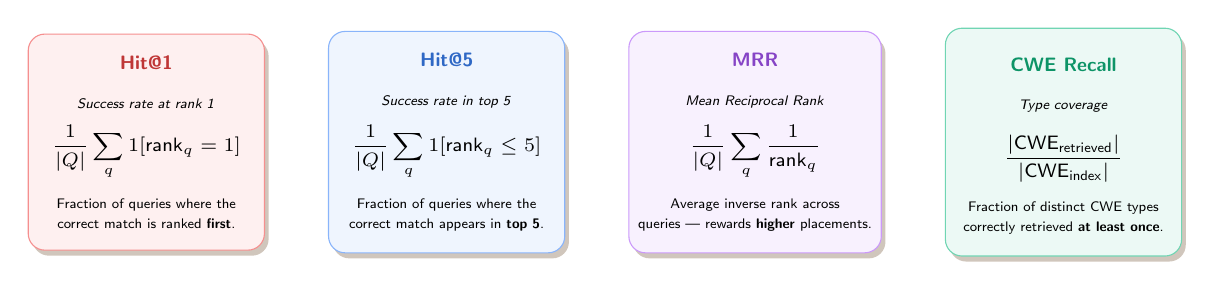
\begin{tikzpicture}[
    node distance=0.6cm and 1.2cm,
    mcard/.style={
      draw=#1!60, fill=#1!8,
      rounded corners=6pt,
      minimum width=3cm,
      minimum height=2.4cm,
      inner ysep=8pt,
      font=\scriptsize\sffamily,
      align=center,
      drop shadow={shadow xshift=1.5pt, shadow yshift=-2pt, opacity=0.3, fill=shadowcol}
    },
    mtitle/.style={
      font=\scriptsize\sffamily\bfseries,
      text=#1!80!black
    },
    micon/.style={
      font=\Large,
      text=#1
    }
  ]

    % --- Card 1: Hit@1 ---
    \node[mcard=ccode] (h1) {
      % \textcolor{ccode}{\faBuilding}\\[4pt]
      {\scriptsize\bfseries\textcolor{ccode!80!black}{Hit@1}}\\[6pt]
      {\tiny\textit{Success rate at rank 1}}\\[5pt]
      $\displaystyle\frac{1}{|Q|}\sum_{q} \mathbbm{1}[\text{rank}_q = 1]$\\[6pt]
      {\tiny Fraction of queries where the}\\[-1pt]
      {\tiny correct match is ranked \textbf{first}.}
    };

    % --- Card 2: Hit@5 ---
    \node[mcard=ccpg, right=0.8cm of h1] (h5) {
      % \textcolor{ccpg}{\faListOl}\\[4pt]
      {\scriptsize\bfseries\textcolor{ccpg!80!black}{Hit@5}}\\[6pt]
      {\tiny\textit{Success rate in top 5}}\\[5pt]
      $\displaystyle\frac{1}{|Q|}\sum_{q} \mathbbm{1}[\text{rank}_q \leq 5]$\\[6pt]
      {\tiny Fraction of queries where the}\\[-1pt]
      {\tiny correct match appears in \textbf{top 5}.}
    };

    % --- Card 3: MRR ---
    \node[mcard=cemb, right=0.8cm of h5] (mrr) {
      % \textcolor{cemb}{\faSortAmountDown}\\[4pt]
      {\scriptsize\bfseries\textcolor{cemb!80!black}{MRR}}\\[6pt]
      {\tiny\textit{Mean Reciprocal Rank}}\\[5pt]
      $\displaystyle\frac{1}{|Q|}\sum_{q} \frac{1}{\text{rank}_q}$\\[6pt]
      {\tiny Average inverse rank across}\\[-1pt]
      {\tiny queries — rewards \textbf{higher} placements.}
    };

    % --- Card 4: CWE Recall ---
    \node[mcard=csub, right=0.8cm of mrr] (cwe) {
      \\[-0.5pt]
      % \textcolor{csub}{\faProjectDiagram}\\[4pt]
      {\scriptsize\bfseries\textcolor{csub!80!black}{CWE Recall}}\\[6pt]
      {\tiny\textit{Type coverage}}\\[7pt]
      $\displaystyle\frac{|\text{CWE}_{\text{retrieved}}|}{|\text{CWE}_{\text{index}}|}$\\[6pt]
      {\tiny Fraction of distinct CWE types}\\[-1pt]
      {\tiny correctly retrieved \textbf{at least once}.}
      % \\[-0.01pt]
    };

  \end{tikzpicture}
  \end{center}
 

\end{frame}
% =====================================================================
% PHASE 1: AUTOPATCH RESULTS
% =====================================================================
\begin{frame}{ AutoPatch Dataset Results (n=225)}
  % \textbf{Goal:} Validate that structural embeddings match CodeBERT performance.

  \vspace{0.3cm}
  \begin{table}
    \centering
    \small
    \begin{tabular}{lrrrr}
      \toprule
      \textbf{Embedder} & \textbf{H@1} & \textbf{H@5} & \textbf{MRR} & \textbf{CWE R.} \\
      \midrule
      \multicolumn{5}{c}{\textit{Structure-Only}} \\
      \midrule
      \textbf{Combined} & \textbf{0.8904} & \textbf{0.9589} & \textbf{0.9162} & \textbf{0.4978} \\
      GIN & 0.7260 & 0.8767 & 0.7879 & 0.4427 \\
      WL & 0.6986 & 0.7945 & 0.7363 & 0.4386 \\
      \midrule
      \multicolumn{5}{c}{\textit{CodeBERT pretrained}} \\
      \midrule
      CodeBERT (baseline) & 0.1533 & 0.2200 & 0.1826 & 0.2933 \\
      CodeBERT (seq) & 0.7534 & 0.8630 & 0.7927 & 0.4121 \\
CodeBERT (pat) & 0.7123 & 0.8356 & 0.7677 & 0.4147 \\      \bottomrule
    \end{tabular}
    \\[2pt]
    {\tiny\textcolor{notecol}{Source: \texttt{experiments/output/checkpoint5/20260505\_141347\_experiment\_f59ab1/results.json}}}
  \end{table}

  
  \textbf{RQ1:} validated — structural \textit{graph} representations are \textit{effective} for vulnerability pattern retrieval in a synthetic dataset.
\end{frame}



% =====================================================================
% PHASE 2: CVEFIXES RESULTS
% =====================================================================
\begin{frame}{CVEfixes Dataset - Input: Function only}
  
  \textbf{Question:} Does the approach generalize to real-world vulnerabilities?
  \vspace{0.3cm}
  
\begin{columns}[T]
\begin{column}{0.48\textwidth}

  \textbf{Real-World Dataset}\\[3pt]
  {\small CVEFixes \cite{bhandari2021cvefixes} datasets is large dataset with real-world CVEs collected from the U.S. National Vulnerability Database, patches, and code changes.\\}
  
  \vspace{0.5em}
  \begin{center}
    
  \scriptsize
  \begin{tabular}{lr}
    \toprule
    \textbf{Metric} & \textbf{Value} \\
    \midrule
    CVEs & 11,873 \\
    Fix commits & 12,107 \\
    File changes & 51,342 \\
    Method changes & 277,948 \\
    Repositories & 4,249 \\
    \bottomrule
  \end{tabular}
  \end{center}
\end{column}
\begin{column}{0.50\textwidth}
    {\small\textbf{Sampling criteria}}\\[3pt]
  {\scriptsize
  \begin{itemize}\itemsep1pt
      \setbeamertemplate{itemize item}{}
    \item Structurally distinshable CWEs (e.g. UAF vs. OOB) to test pattern matching, not just code similarity
    \item Balanced superclass(CWE) up to 20 entries and subclasses (CVE) to ensure retrieval feasibility
  \end{itemize}}
      \vspace{0.5em}
    \begin{center}

  {\scriptsize
  \renewcommand{\arraystretch}{1.2}
  \begin{tabular}{lr}
    \toprule
    \textbf{Parameter} & \textbf{Value} \\
    \midrule
    Total pairs & 136 \\
    Index set & 109 \\
    Query set & 27 \\
    Unique CVEs (index) & 60 \\
    Unique CVEs (query) & 25 \\
    CWE classes & 7 \\
    % Slice depth & 2-hop \\
    % Min/max lines & 10 / 120 \\
    \bottomrule
  \end{tabular}}

    \end{center}
  
\end{column}
\end{columns}
\end{frame}


\begin{frame}{Results}

  \begin{columns}[T]
    \begin{column}{0.5\textwidth}

  \begin{center}
    {\small\textbf{Same-CWE Retrieval} {\scriptsize(n=109 index, 27 query)}}\\[6pt]
  {\scriptsize
  \renewcommand{\arraystretch}{1.35}
  \setlength{\tabcolsep}{3.5pt}
    \begin{tabular}{lrrrr}
      \toprule
      \textbf{Embedder} & \textbf{Hit@1} & \textbf{Hit@5} & \textbf{MRR} & \textbf{CWE Recall} \\
      \midrule
      GIN & 0.259 & 0.778 & 0.315 & 0.202 \\
      \rowcolor{warn!12}
      Combined & \cmiss{0.111} & 0.778 & 0.223 & 0.189 \\
      CodeBERT (baseline) & 0.080 & 0.1518 & 0.098 & 0.141 \\
      \rowcolor{hit!12}
      \textbf{CodeBERT (seq)} & \textbf{0.556} & \textbf{0.926} & \textbf{0.555} & \textbf{0.264} \\
      \textbf{CodeBERT (pat)} & \textbf{0.519} & \textbf{0.889} & \textbf{0.549} & \textbf{0.276} \\
      \bottomrule
    \end{tabular}
  }

  \vspace{0.3em}
  {\tiny\textcolor{notecol}{Source: \texttt{cvefixes\_experiments/output/pipeline\_verification/results.json}}}

  
  \end{center}
  
    \end{column}
    \begin{column}{0.5\textwidth}

  \begin{center}
  {\small\textbf{Per-CWE Breakdown} {\scriptsize(CodeBERT Pattern, CWE Hit@$k$)}}\\[6pt]
  {\scriptsize
  \renewcommand{\arraystretch}{1.35}
  \setlength{\tabcolsep}{3.5pt}
  \begin{tabular}{l r rrr}
    \toprule
    \textbf{CWE} & \textbf{N} & \textbf{Hit@1} & \textbf{Hit@5} & \textbf{Hit@10} \\
    \midrule
    Integer Overflow (190) & 4 & \chit{75\%} & 100\% & 100\% \\
    Input Validation (20) & 4 & \chit{75\%} & 75\% & 100\% \\
    Resource Consump.\ (400) & 3 & \chit{67\%} & 100\% & 100\% \\
    Use After Free (416) & 4 & 50\% & 100\% & 100\% \\
    NULL Ptr Deref (476) & 5 & \cwarn{40\%} & 80\% & 80\% \\
    Race Condition (362) & 3 & \cwarn{33\%} & 100\% & 100\% \\
    OOB Write (787) & 4 & \cmiss{25\%} & 75\% & 75\% \\
    \midrule
    \textbf{Overall} & \textbf{27} & \textbf{51.9\%} & \textbf{88.9\%} & \textbf{92.6\%} \\
    \bottomrule
  \end{tabular}}

  \vspace{0.2em}
  {\tiny\textcolor{notecol}{Source: same file (CodeBERT Pattern cell)}}

  \vspace{0.2em}
  {\scriptsize\textcolor{notecol}{Highlights areas for improvement in embedding design or slicing strategy.}}
  \end{center}
    \end{column}
  \end{columns}
\end{frame}

\begin{frame}{Results for File as Input }

  \begin{columns}[T]
    \begin{column}{0.58\textwidth}

  \begin{center}
    {\small\textbf{Retrieval by Graph Input Type (CVE)} {\scriptsize(n=132 index, 8 query)} }\\[4pt]
  {\scriptsize
  \renewcommand{\arraystretch}{1.22}
  \setlength{\tabcolsep}{3.2pt}
    \begin{tabular}{llrrrr}
      \toprule
      \textbf{Graph input} & \textbf{Embedder} & \textbf{Hit@1} & \textbf{Hit@5} & \textbf{MRR} & \textbf{CWE R.} \\
      \midrule
      \multicolumn{6}{l}{\textit{G\_vuln: vulnerability-focused subgraph}} \\
      G\_vuln & Combined & 0.500 & 0.750 & 0.603 & 0.194 \\
      G\_vuln & CodeBERT (seq) & 0.500 & 0.750 & 0.573 & 0.269 \\
      G\_vuln & \textbf{CodeBERT (pat)} & \textbf{0.500} & \textbf{1.000} & \textbf{0.656} & \textbf{0.331} \\
      \midrule
      \multicolumn{6}{l}{\textit{G\_before: full pre-patch file}} \\
      G\_before & Combined & 0.125 & 0.125 & 0.179 & 0.238 \\
      G\_before & \textbf{CodeBERT (seq)} & \textbf{0.625} & \textbf{1.000} & \textbf{0.792} & \textbf{0.350} \\
      G\_before & CodeBERT (pat) & 0.375 & 0.875 & 0.594 & 0.250 \\
      \bottomrule
    \end{tabular}}
  \end{center}

  \vspace{0.35em}
  \begin{tcolorbox}[colback=warn!5, colframe=warn!70!black, boxrule=0.35pt,
    left=3pt, right=3pt, top=2pt, bottom=1pt, arc=2pt, width=\linewidth]
    \scriptsize
    \textit{G\_vuln} sharpens the vulnerability signal, this increase the preprocessing but allows simple graph pattern to retrieve the vulnerability more correctly.
    \textit{G\_before} keeps the full pre-patch file context, which helps CodeBERT sequence models recover more hits, but the broader context weakens the graph signal.


  \end{tcolorbox}

    \end{column}
    \begin{column}{0.42\textwidth}

  \begin{center}
  {\small\textbf{Combined on G\_vuln: Per-CWE Hit@k}}\\[4pt]
  {\scriptsize
  \renewcommand{\arraystretch}{1.25}
  \setlength{\tabcolsep}{3.2pt}
  \begin{tabular}{lrrrr}
    \toprule
    \textbf{CWE} & \textbf{N} & \textbf{Hit@1} & \textbf{Hit@5} & \textbf{Hit@10} \\
    \midrule
    CWE-476 & 1 & 0.000 & 0.000 & \chit{1.000} \\
    CWE-362 & 2 & \chit{0.500} & \chit{0.500} & 0.500 \\
    CWE-400 & 4 & \chit{0.750} & \chit{1.000} & \chit{1.000} \\
    CWE-190 & 1 & 0.000 & \chit{1.000} & \chit{1.000} \\
    \midrule
    \textbf{Overall} & \textbf{8} & \textbf{0.500} & \textbf{0.750} & \textbf{0.875} \\
    \bottomrule
  \end{tabular}}

  \vspace{0.2em}
  {\scriptsize\textcolor{notecol}{From run \texttt{20260629\_165056\_cvefixes\_retrieval\_grid\_f05322}}}
  \end{center}
    \end{column}
  \end{columns}
\end{frame}


\begin{frame}{Results for File as Input (Larger Dataset)}


  \begin{center}
    {\small\textbf{Retrieval by Graph Input Type (CVE)} {\scriptsize(n=439 index, 113 query)} }\\[4pt]
  {\scriptsize
  \renewcommand{\arraystretch}{1.22}
  \setlength{\tabcolsep}{3.2pt}
    \begin{tabular}{llrrrr}
      \toprule
      \textbf{Graph input} & \textbf{Embedder} & \textbf{Hit@1} & \textbf{Hit@5} & \textbf{MRR} & \textbf{CWE R.} \\
      \midrule
      \multicolumn{6}{l}{\textit{G\_vuln: vulnerability-focused subgraph}} \\
      G\_vuln & Combined & 0.292 & 0.434 & 0.0357 & 0.218 \\
      G\_vuln & CodeBERT (seq) & 0.602 & 0.752 & 0.0670 & 0.336 \\
      G\_vuln & CodeBERT (pat) & 0.496 & 0.673 & 0.575 & 0.322 \\
      \midrule
      \multicolumn{6}{l}{\textit{G\_before: full pre-patch file}} \\
      G\_before & Combined & 0.044 & 0.204 & 0.125 & 0.164 \\
      G\_before & \textbf{CodeBERT (seq)} & \textbf{0.549} & \textbf{0.735} & \textbf{0.618} & \textbf{0.314} \\
      G\_before & CodeBERT (pat) & 0.522 & 0.699 & 0.594 & 0.302 \\
      \bottomrule
    \end{tabular}}

     \vspace{0.2em}
  {\scriptsize\textcolor{notecol}{From runs:\\
  \texttt{Vulnerability: 20260629\_100842\_cvefixes\_retrieval\_grid\_060f17}\\
  \texttt{Before: 20260629\_143613\_cvefixes\_retrieval\_grid\_4c44f8}}}
  \end{center}

\end{frame}


% ── closing ───────────────────────────────────────────────────────────
\begin{frame}[plain]
\centering
\vspace{3em}
{\LARGE\bfseries\color{c1} Questions?}\\[2em]

\begin{tikzpicture}
  \node[draw=c1!30, rounded corners=6pt, fill=c1!5,
        minimum width=9cm, minimum height=1.4cm,
        font=\small\sffamily\color{notecol}, align=center]
    {Lívia Cavalcanti\quad\textbar\quad\faIcon{github}\ \texttt{graph-rag/}};
\end{tikzpicture}
\end{frame}

\end{document}


%  \begin{center}
%   {\small\textbf{G\_vuln Per-CWE Recall}}\\[4pt]
%   {\scriptsize
%   \renewcommand{\arraystretch}{1.25}
%   \setlength{\tabcolsep}{4pt}
%   \begin{tabular}{lrrr}
%     \toprule
%     \textbf{CWE} & \textbf{Seq} & \textbf{Pat} & \textbf{Comb.} \\
%     \midrule
%     CWE-476 & 0.000 & 0.100 & \chit{0.200} \\
%     CWE-362 & \chit{0.250} & 0.200 & 0.200 \\
%     CWE-400 & 0.525 & \chit{0.725} & 0.275 \\
%     CWE-190 & \chit{0.300} & \chit{0.300} & 0.100 \\
%     \midrule
%     \textbf{Macro avg.} & \textbf{0.269} & \textbf{0.331} & \textbf{0.194} \\
%     \bottomrule
%   \end{tabular}}